\documentclass{article}
\usepackage{factsheet}

\begin{document}
% Cover Page

\begin{titlepage}
	\centering
    \vfill
    \vspace{3cm}
	{\huge\bfseries Project Proposal\par}
    {\Large Project ID: MR02a-24\par}
	\vspace{2cm}
	{\Large Ujaan Das ID: 20796435\\
                    Armaan Dayal ID: 20794138\\
                    Wiktor Kowalczyk ID: 2081409\\}

	\vfill
	{\large \today\par}
    \vspace{5cm}
    \rule{\textwidth}{0.4pt}
    \begin{itemize}
    \item Design and fabricate a self-mobile robot capable of omnidirectional floor movement, equipped to carry required electrical components.
    \item Develop a system capable of following a specified individual within a 1m distance.
    \item Integrate the person-tracking algorithm with the robot’s navigation system to enable the robot to follow the individual through crowds and potential occlusions.
    \item Implement facial recognition technology to identify patients with >90\% accuracy.
    \item Engineer a dispensing mechanism that accurately enables retrieval of the correct medication for the identified patient.
    \item Integrate the above systems in tandem to meet final project goal.
    \end{itemize}

\end{titlepage}
% Table of Contents
\tableofcontents
\thispagestyle{empty}
\newpage

% Arabic numerals for content pages
\pagenumbering{arabic}

% Section 1 Introduction
\section{Introduction}
\subsection{Background and Engineering Problem}
The public healthcare system in Hong Kong is currently facing a significant crisis characterized by a critical shortage of nursing staff. This issue has been exacerbated by numerous factors in recent years, including an aging population and the aftermath of the COVID-19 pandemic. As of 2022, there were approximately 66,492 nurses in Hong Kong, but projections suggest a growing shortfall, with estimates indicating a deficit of around 3,000 general nurses by 2030 and up to 5,000 by 2040 \cite{lam2022shortage}. The role of nurses in patient care is critical, particularly in administering medications. Currently, nurses spend a considerable amount of time verifying patient identities and retrieving medications from dispensing areas. This repetitive task of moving between patients' beds and the medication area leads to delays in patient care and increased workloads for nursing staff, further contributing to burnout and attrition rates.

To address these challenges, we propose the development of a nurse-following robot designed to assist nurses in medication administration. At each bed, the robot will scan the patients' faces to identify them, then allow the nurse to retrieve the correct medication for that patient. The engineering problems associated with this project include developing a robust and mobile robot capable of following a nurse through the hospital environment, implementing a reliable facial recognition system that ensures accurate patient identification, and designing a mechanism that allows the efficient retrieval of the correct medications.

\subsection{Objectives}
% Minimum ¼ page
This project aims to design and build a person-following robot and apply it to the context of a hospital to follow nurses. Equipped with advanced navigation, tracking, and facial recognition capabilities, the robot will autonomously navigate healthcare environments, identify patients, and dispense the correct medication, thereby enhancing patient care efficiency and accuracy.

\subsubsection{Objective Statements}
\begin{enumerate}
    \item Design and fabricate a self-mobile robot capable of omnidirectional floor movement, equipped to carry required electrical components.
    % \item Develop an obstacle avoidance system for the robot that achieves at least an 85\% success rate in navigating to a predetermined point without collisions.
    \item Develop a system capable of following a specified individual within a 1m distance.
    \item Integrate the person-tracking algorithm with the robot’s navigation system to enable the robot to follow the individual through crowds and potential occlusions.
    \item Implement facial recognition technology to identify patients with >90\% accuracy.
    \item Engineer a dispensing mechanism that accurately enables retrieval of the correct medication for the identified patient.
    \item Integrate the above systems in tandem to meet final project goal.
\end{enumerate}

\subsection{Literature Review of Existing Solutions}
% Minimum 1 page
In the past, numerous implementations utilized basic micro controllers in their designs as the main computation and decision device \cite{ilias2014hospital}. This approach has the benefits of being cheap and having an established community of maintained open-sources libraries. However, the significant drawback is the limited computational power of such a setup. Increased computational capabilities are becoming cheaper and cheaper, allowing us to use more sophisticated algorithms that enable new and more accurate navigation methods. One way of increasing the capabilities of a system in the past implementations was to use a portable personal computer as the main computation hub \cite{ilias2014nurse}\cite{kautsar2019simple}. This approach introduces certain drawbacks. It increases the weight of the system, reduces possible payload space, and escalates the complexity of the system with regards to the control of peripheral hardware. Our system relies on Raspberry Pi 5 which is the middle ground between microcontrollers and portable personal computers. It offers great computing power in a small and light package, simultaneously enabling us to use software abstractions of hardware control while retaining low-level understanding and control of the system peripherals.

Additionally, the ability for a robotic system to track and follow a specific person would invite a wide array of applications, such as assistive technologies (which we are currently exploring), surveillance, and Human-Computer Interaction (HCI). However, and due to the inherent breadth of the topic and the approaches thereof, most solutions can be split into 2 categories, those reliant on Electro-Magnetic (EM) waves and a tagging system, such as Infrared (IR) or Ultra-wideband (UWB), and those utilizing machine learning algorithms to categorize features such as You Only Look Once (YOLO) and Simple Online Realtime Tracking (SORT/DeepSORT).

UWB systems, while still relatively novel in consumer applications, are widely recognized for their high accuracy in indoor positioning. As the name suggests, they operate by transmitting signals across a wide spectrum of frequencies, which thereby enhance their ability to measure distances precisely. The tags are small, low power, and can be easily attached/placed on a person, allowing our robot to follow along with ease \cite{zhang2009uwb}. Thus, UWB systems outperform many other localization techniques in terms of accuracy, especially indoors, and are also less susceptible to interference from other signals \cite{zhang2009uwb} \cite{alarifi2016ultra}. However, this approach would mandate a robust form of velocity approximation via Kalman filtering or something else, as UWB performance is known to degrade in non-line-of-sight conditions, thus limiting effectiveness in cluttered environments such as those of a hospital \cite{alarifi2016ultra}.

On the other hand, popular machine learning/computer vision approaches have shown significant promise in person-following applications, with the bulk of similar research papers utilizing YOLO and Simple Online and Realtime Tracking (SORT) derivations. YOLO is a real-time object detection system that is highly efficient and capable of detecting multiple objects of multiple given classes in a single frame. Its unified architecture allows it to process images quickly, thereby being very suitable for real-time applications where speed is critical \cite{han2021you}. However, and even barring any trade-offs in accuracy, YOLO alone will not be sufficient, as we will need to implement further re-identification models to allow the robot to resume following after any given partial occlusion or losses in vision (ie; sharp turns) \cite{han2021you}. Thus, approaches such as SORT and DeepSORT were also considered, which combine deep learning for object detection with a Kalman filter for trajectory estimation, which allows for robust tracking and consistent identification even in crowded scenes \cite{wojke2017simple}. Still, the combination of detection, tracking and re-identification can introduce a large computational overhead, and might lead to slowdowns on less powerful hardware, ie; our Raspberry Pi 5 \cite{wojke2017simple}.

% Section 2 Methodology
\section{Methodology}

\subsection{Overview}

\subsubsection{System Description}
% Minimum ½ page
The main design pattern for this robot is a tower structure with three wheels. The base of the robot will consist of core electronic components including the battery, motors and their encoders, driver circuits, and essential computing hardware. The carriage will include three motors with Swedish 90\degree wheels in a triangular configuration to allow full omnidirectional movement.
Another layer will be built above this, which will carry the medication access mechanism and environment scanning sensors, including the camera and LIDAR sensor. Presently, we envisage the medication access mechanism to consist of an array of electromagnetic locks that hold pre-dispensed medication in paper cups.

The power supply consists of wall AC-DC adapter which allows us to disregard complexities that arise from battery-powered design, however, the DC bus is designed to allow interchangeability between Lithium Ion batteries and a cable supply. As shown in Fig. \ref{fig:block_diagram}, the power source is connected to the DC terminal from which we wire two separate DC-DC converters. One is for providing suitable power and voltage to the logic circuits, and the other for supplying adequate voltage and current to the DC motors. This design ensures full decoupling between low current logic circuits and high current and high volatility motors circuits, ensuring stable supply for both systems. However, our main goal is to use lithium ion battery packs as the main power supply since they enable the robot to move freely around the hospital.

The main software architecture is based on the Robot Operating System 2 (ROS2) on Ubuntu 24.04 Noble Numbat. It allows us to abstract hardware interfaces while maintaining lower-level control; ROS2 also provides a set of patterns to base our system design on. In our design we will utilize a node-based approach, where each node is a single entity responsible for controlling one piece of hardware or doing one set of adjacent computations. The nodes will then communicate between themselves on a server-client basis using a set of message types defined by us beforehand. This approach introduces additional modularity, enabling easier testing and prototyping of different parts of the system.



\subsubsection{System Block Diagram}
\begin{figure}[H]
    \centering
    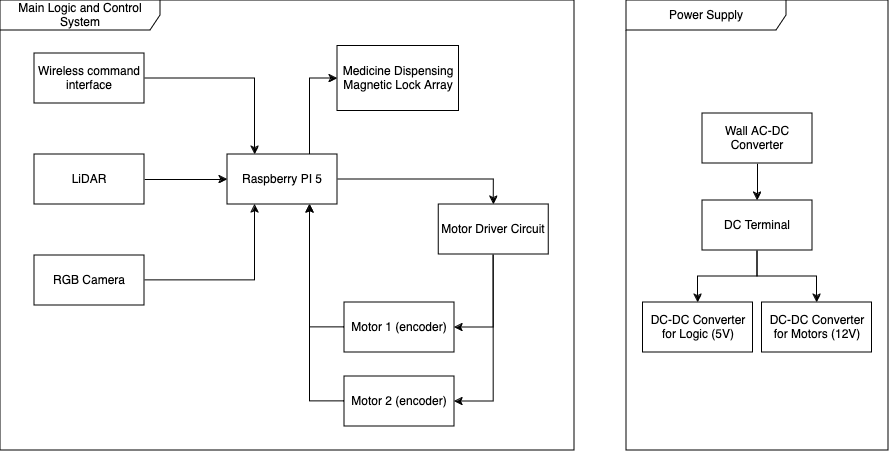
\includegraphics[width=0.8\textwidth]{media/FYP-block-diagram.png} % Placeholder for your block diagram image
    \caption{Block diagram of the main system components.}
    \label{fig:block_diagram}
\end{figure}

\subsubsection{Components List}
\begin{table}[H]
    \centering
    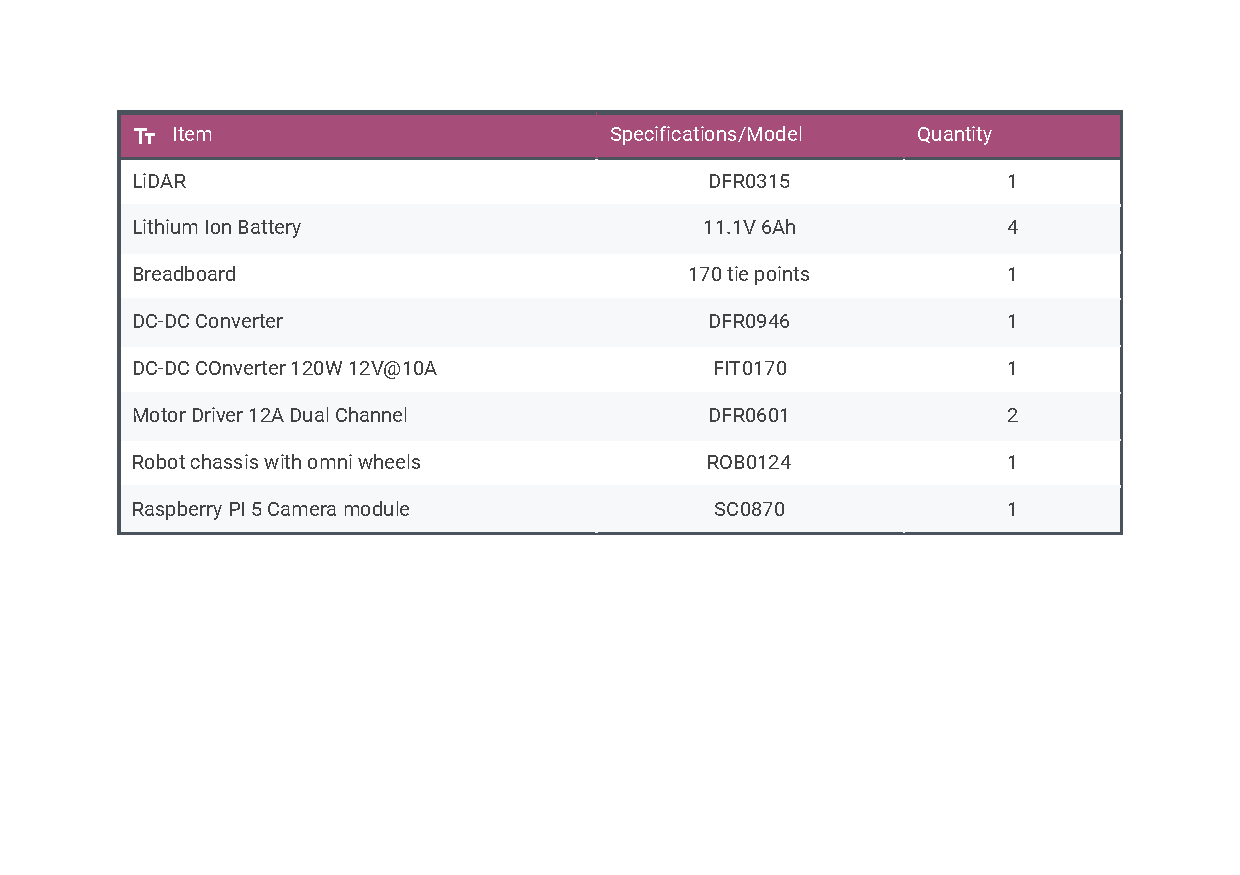
\includegraphics[width=0.5\textwidth]{media/ProjectBudget - Arkusz3.pdf} % Placeholder for your block diagram image
    \caption{Main component list.}
    \label{table:component_list}
\end{table}
\subsubsection{ECE Knowledge}
% Minimum ½ page
In our project we extensively utilize knowledge from many ECE and COMP courses, be it required courses or electives:
\begin{itemize}
    \item ELEC 2400 Electronic Circuits -- This course taught us the basics of electronic circuits which will aid us in designing the power supply system for our robot.
    \item ELEC 3300 Introduction to Embedded Systems -- From this course we learnt project planning in the context of integrating embedded systems. This knowledge is foundational to this project.
    \item ELEC 3210 Introduction to Mobile Robotics -- This course is the basis of our navigation and mapping subsystems. It also taught us how to use Robot Operating System which we also utilise in our project.
    \item COMP 2011 Programming with C++ -- Provided us with fundamental knowledge of programming.
    \item COMP 2012 Object Oriented Programming and Data Structures -- Provided us with fundamental knowledge in data organization and object oriented approach to system design which we utilize in our Robot Operating System approach.
\end{itemize}

\subsection{Objective Statement Execution}
% Minimum 2 pages
\begin{enumerate}
    \item \textbf{Design and fabricate a self-mobile robot capable of omnidirectional floor movement, equipped to carry required electrical components.}\\
Tasks:
\begin{enumerate}
    \item Design the robot’s base and wheel system for omnidirectional movement.
%Armaan:
\begin{enumerate}
    \item Create/design a robot chassis that would support omnidirectional movement. This involves selecting appropriate wheel types, such as regular, Mecanum or omni-wheels, to allow smooth and flexible navigation, as well as an appropriate shape, layer structure, turning mechanism.
\end{enumerate}

\item Select and integrate motors and motor controllers suitable for the design.
%Wiktor:
Choose motors and controllers that are compatible with the chosen wheel system design. 
\begin{enumerate}
    \item Ensure the motors provide sufficient torque and speed given our projected weight/speed/duration estimates. Also integrate motor controllers to facilitate precise control over movement, as well as testing the setup for responsiveness and reliability.
\end{enumerate}

\item 
Design and implement the power distribution system, including battery placement and wiring.
\begin{enumerate}
    \item Develop a power distribution system to efficiently deliver power to all components. Focus on battery selection and placement, wiring design, and implementing safety features. Further test the system for load management and efficiency.
\end{enumerate}
%Ujaan:

\item 
Mount and secure the additional layers, LiDAR sensor, camera and other peripheral components.
\begin{enumerate}
    \item Securely mount the LiDAR sensor, camera, and other peripherals (or equally sized/weighted mocks thereof) onto the robot. Also design mounts that minimize vibration and ensure stable data collection. Proper alignment and calibration will be performed to optimize performance. 
\end{enumerate}
%Wiktor:

\item 
Test the robot’s movement capabilities and make necessary adjustments.
\begin{enumerate}
    \item Conduct tests to evaluate the robot's movement capabilities. Also set up various tracks and courses to assess the robot’s ability to maneuver and make necessary adjustments if needed to improve performance.
\end{enumerate}
%Armaan:

\end{enumerate}

% \item \textbf{Develop an obstacle avoidance system for the robot that achieves at least an 85\% success rate in navigating to a predetermined point without collisions.}\\
% The objective is to allow the currently-basic robot to perform the necessary object detection and navigations that would be required in a crowded hospital scenario. It should be capable of making rapid course corrections, sharp right angle turns, backtracking, and whatever else is required.\\
% Tasks:
% \begin{enumerate}
%     \item Develop and implement sensor fusion algorithms to combine data from multiple sensors.
%     %Wiktor: 
%     Create algorithms to combine data from multiple sensors like LiDAR and ultrasonic. Focus on enhancing data accuracy and reliability, ensuring the robot can detect and respond to obstacles effectively.
%     \item Use ROS2 Jazzy to program the robot’s navigation software to process sensor data and detect obstacles.
%     %Wiktor: 
%     Utilize ROS2 Jazzy to develop the robot's navigation software. Program the robot to process sensor data and detect obstacles, implementing a user-friendly interface for smooth operation.
%     \item Implement path planning and Simultaneous Localization and Mapping (SLAM) algorithms to navigate around detected obstacles.
%     %Wiktor: 
%     Integrate path planning and SLAM algorithms to enable the robot to navigate around obstacles. Conduct basic simulations to refine these algorithms.
%     \item Perform real-world testing and any necessary refinements.
%     %Armaan: 
%     Test the obstacle avoidance system in real environments. Analyze performance data to identify any issues and make necessary refinements, ensuring an ultimate 85\% success rate in obstacle avoidance.
% \end{enumerate}

\item \textbf{Develop a system capable of following a specified individual within a 1m distance.}\\
The objective is to follow a specific individual (i.e. a nurse) with leeway of at least 1 meter, through lesser degrees of occlusion, and simple turning.\\
Tasks:
\begin{enumerate}
    \item Select and configure a suitable tracking device to be placed on the individual.
    \begin{enumerate}
        \item Choose a suitable tracking device for the individual and configure it for seamless operation. Ensure the device works effectively within a 1-3m range and handle all of the aforementioned challenges.
    \end{enumerate}
    %Ujaan: 
    
    \item Develop the software to receive and process signals from the tracking device.
    \begin{enumerate}
        \item Create software to process signals from the tracking device, and map it to 3D point coordinates to be later implemented with the robot’s navigation system. Focus on consistency and reliability across various ranges and occlusions.
    \end{enumerate}
    %Ujaan: 
    
    % \item Implement algorithms to maintain a consistent lock on the tracking device’s signal.
    % \begin{enumerate}
    %     \item Consider utilizing algorithms such as the Kalman filter or velocity approximation to aid in predicting the appropriate direction the tracked person will travel in cases of occlusion or sharp turns.
    % \end{enumerate}
    %Ujaan: 
    
    \item Test the tracking system in controlled environments with varying conditions.
    \begin{enumerate}
        \item Conduct tests in controlled environments to evaluate the tracking system's performance. Gather data on system accuracy and adjust algorithms as needed.
    \end{enumerate}
    %Armaan: 
    
\end{enumerate}

\item \textbf{Integrate the person-tracking algorithm with the robot’s navigation system to enable the robot to follow the individual through crowds and around obstacles, even with potential occlusions.}\\
Integrate the person-tracking algorithm with the robot’s navigation system: The goal is to seamlessly integrate the person-tracking algorithm with the robot’s navigation system, allowing it to adeptly follow the designated individual through dense crowds and navigate around obstacles, even when facing potential occlusions.\\
Tasks:
\begin{enumerate}
    \item Develop an interface to connect the tracking system with the robot’s navigation software.
    \begin{enumerate}
        \item Create an interface to connect the tracking system with the robot’s navigation software. Ensure smooth data flow and compatibility between systems.
    \end{enumerate}
    %Ujaan: 
    
    \item Implement distance calculation algorithms to maintain an optimal following distance.
    %Ujaan: 
    \begin{enumerate}
        \item Develop algorithms to maintain optimal following distance. Test and refine these algorithms to ensure the robot follows individuals accurately, even in crowds.
    \end{enumerate}
    
    \item Test the integrated system in controlled environments with dynamic obstacles.
    \begin{enumerate}
        \item Evaluate the integrated system in dynamic environments with obstacles and crowds. Analyze performance and make necessary adjustments to improve reliability.
    \end{enumerate}
    %Armaan:  
    
\end{enumerate}

\item \textbf{Implement facial recognition technology to identify patients with >90\% accuracy.}\\
Develop and deploy facial recognition technology to accurately identify individuals and retrieve their medical information from an existing patient database, achieving an accuracy rate of over 90\%.\\
Tasks:
\begin{enumerate}
    \item Develop and train a facial recognition model using a relevant dataset.
    \begin{enumerate}
        \item Train a facial recognition model using a relevant dataset. Focus on optimizing accuracy and speed, ensuring the system meets the >90\% accuracy target.
    \end{enumerate}
    %Armaan: 

    \item Implement a mock patient database with CRUD for information retrieval.
    \begin{enumerate}
        \item Create a mock database and minimal API backend with CRUD functionalities for testing information retrieval. Ensure the system can retrieve data quickly and reliably.
    \end{enumerate}
    %Ujaan: 
    
    \item Test the facial recognition system for accuracy and reliability.
    %Armaan: 
    \begin{enumerate}
        \item Test the facial recognition system for accuracy and reliability. Conduct tests using diverse facial images to ensure consistent performance.
    \end{enumerate}
    
\end{enumerate}

\item \textbf{Engineer a dispensing mechanism that accurately enables retrieval of the correct medication for the identified patient.}\\
Design a precise dispensing mechanism that reliably provides the correct medication to the identified patient, ensuring accuracy and safety in medication distribution.\\
Tasks:
\begin{enumerate}
    \item Design the mechanical components of the dispensing mechanism.
    %Armaan: 
    \begin{enumerate}
        \item Design the mechanical parts of the dispensing mechanism. Focus on precision and reliability, ensuring the mechanism can dispense medication accurately with little lag.
    \end{enumerate}
    
    \item Develop the software to control the dispensing process based on patient identification.
    %Ujaan: 
    \begin{enumerate}
        \item Create software to manage the dispensing process based on patient identification (ie; connecting it to the aforementioned API). Test the system to ensure it dispenses the correct medication without errors.
    \end{enumerate}

    \item Test the dispensing mechanism for accuracy and reliability.
    %Armaan: 
    \begin{enumerate}
        \item Conduct tests to evaluate the accuracy and reliability of the dispensing mechanism. Refine the system as needed to ensure consistent performance.
    \end{enumerate}
    
\end{enumerate}
\end{enumerate}


% Section 3 Project Planning
\begin{landscape}
\section{Project Planning}

\subsection{Project Schedule}

\begin{table}[H]
    \centering
    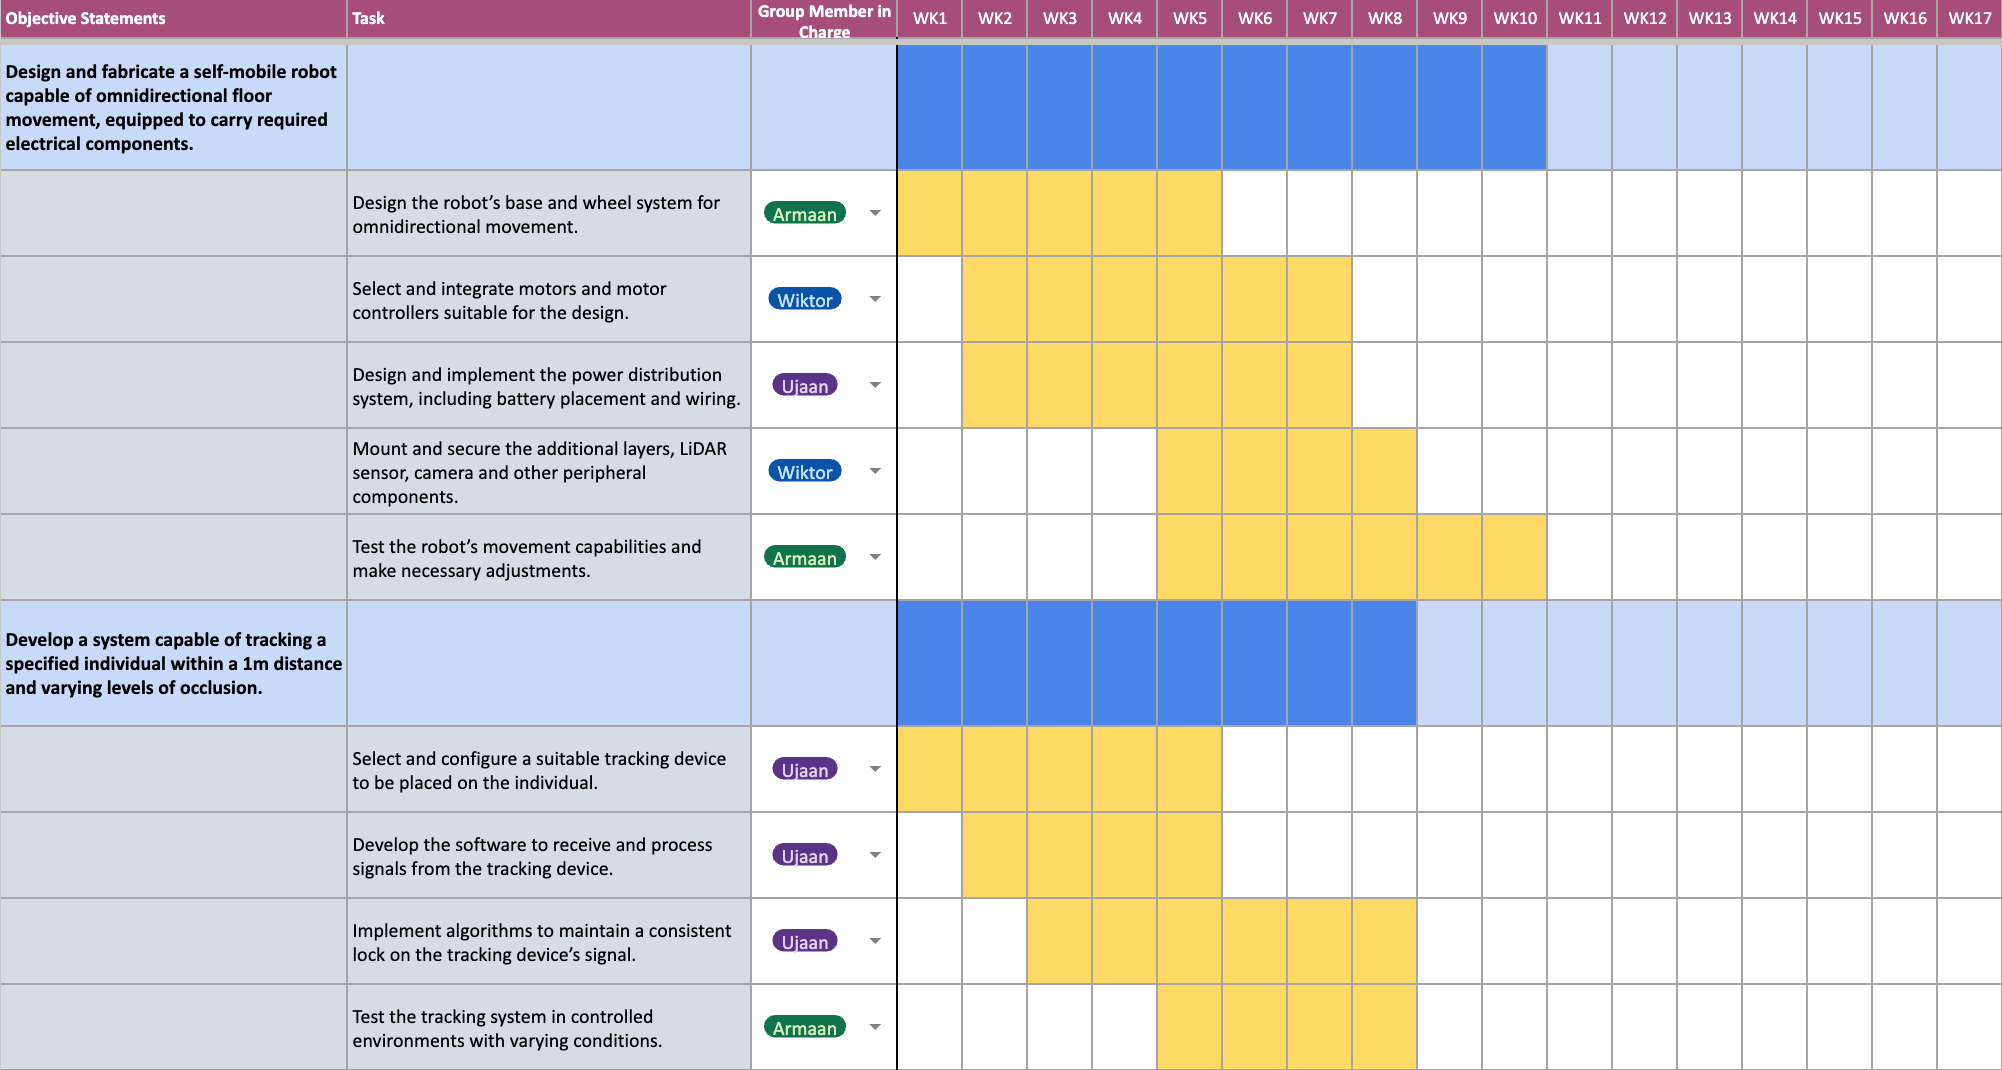
\includegraphics[width=1.2\textwidth]{media/gantt-1.png}
\end{table}
\begin{table}[H]
    \centering
    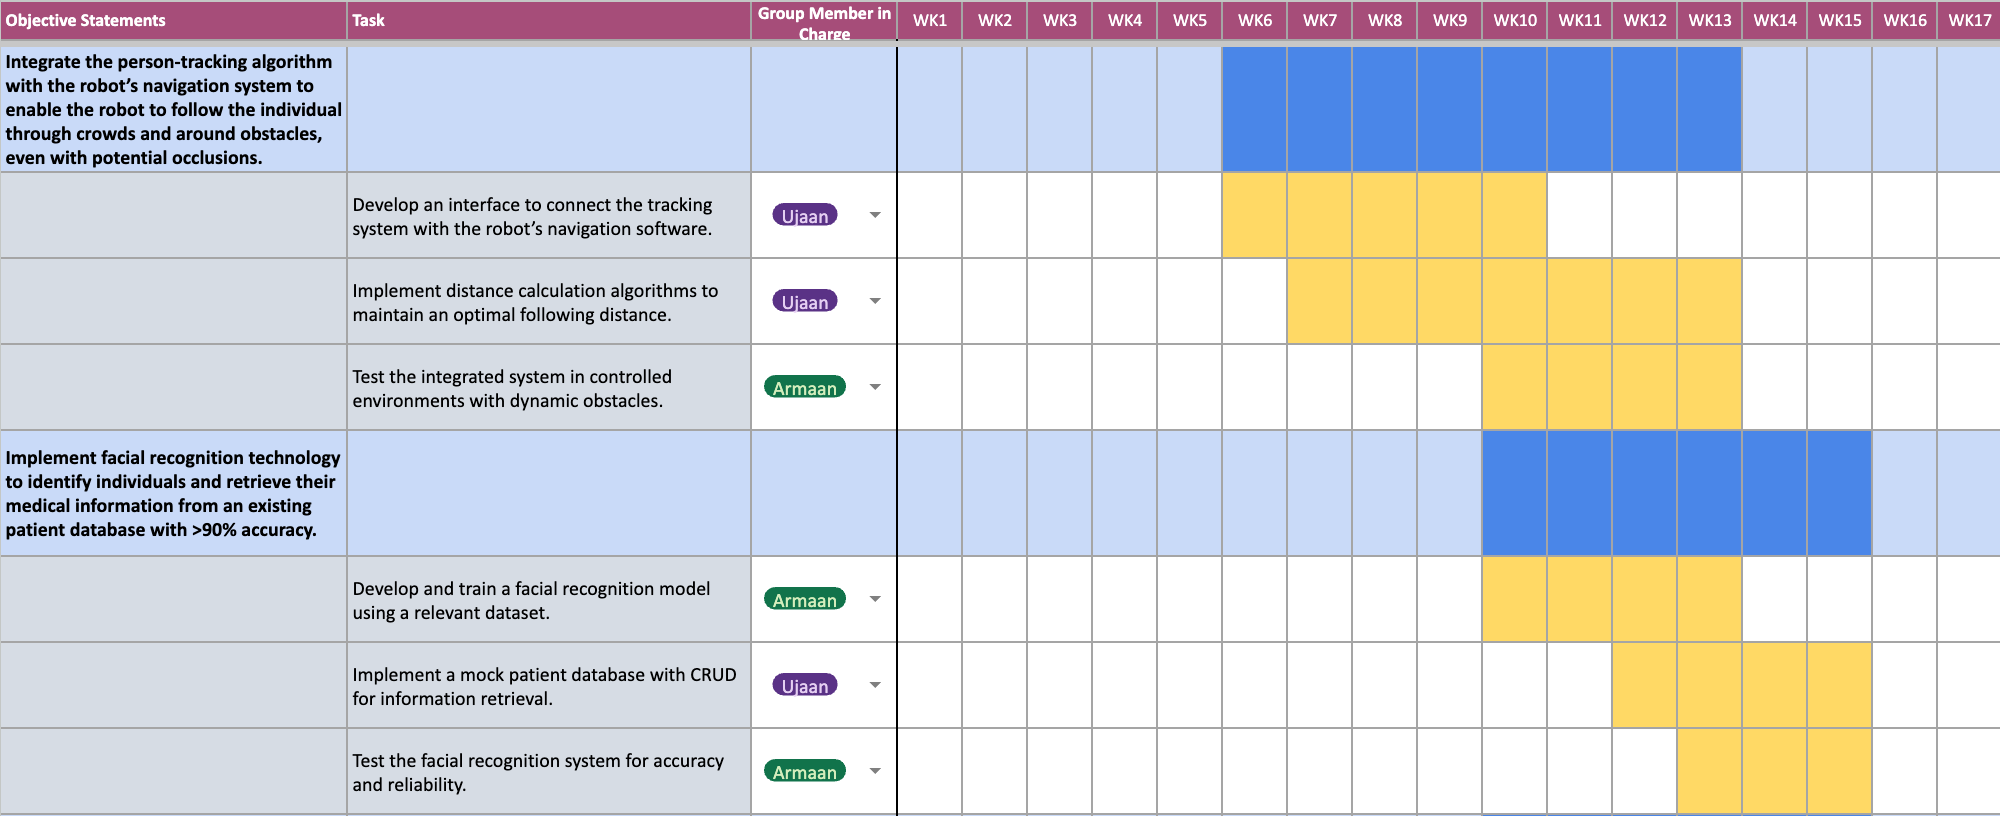
\includegraphics[width=1.2\textwidth]{media/gantt-2.png}
    
    \label{table:gantt_chart}
\end{table}
\begin{table}[H]
    \centering
    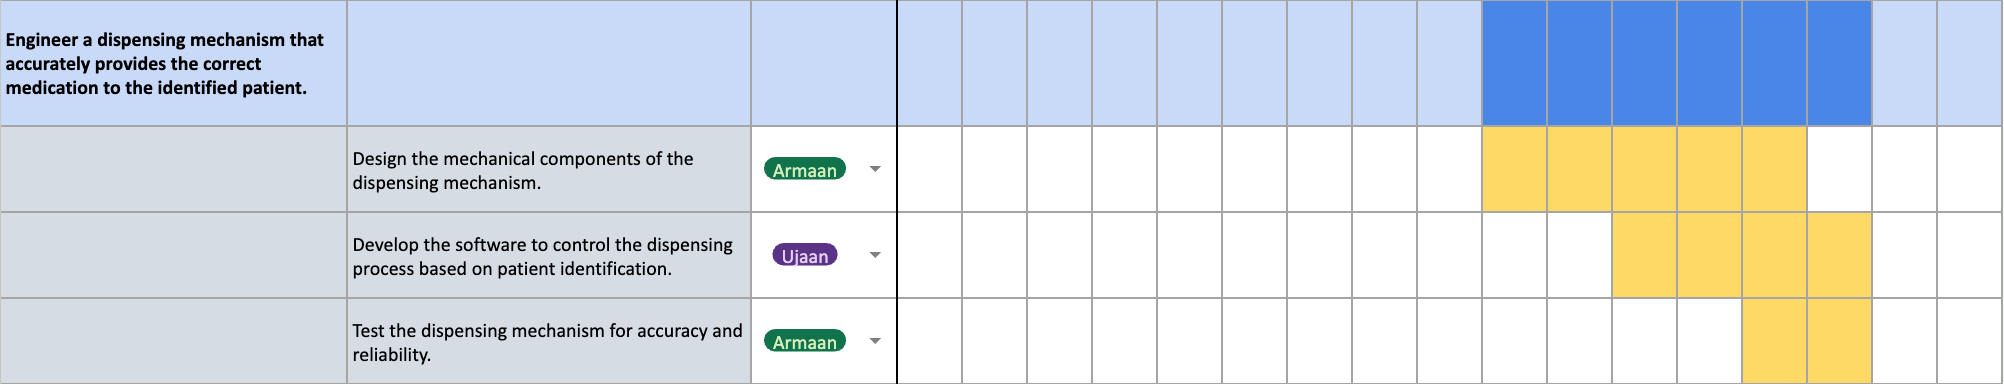
\includegraphics[width=1.2\textwidth]{media/gantt-3.png}
    \caption{Gantt chart of the project timeline.}
    \label{table:gantt_chart}
\end{table}
\end{landscape}

\subsection{Budget}
\begin{table}[H]
    \centering
    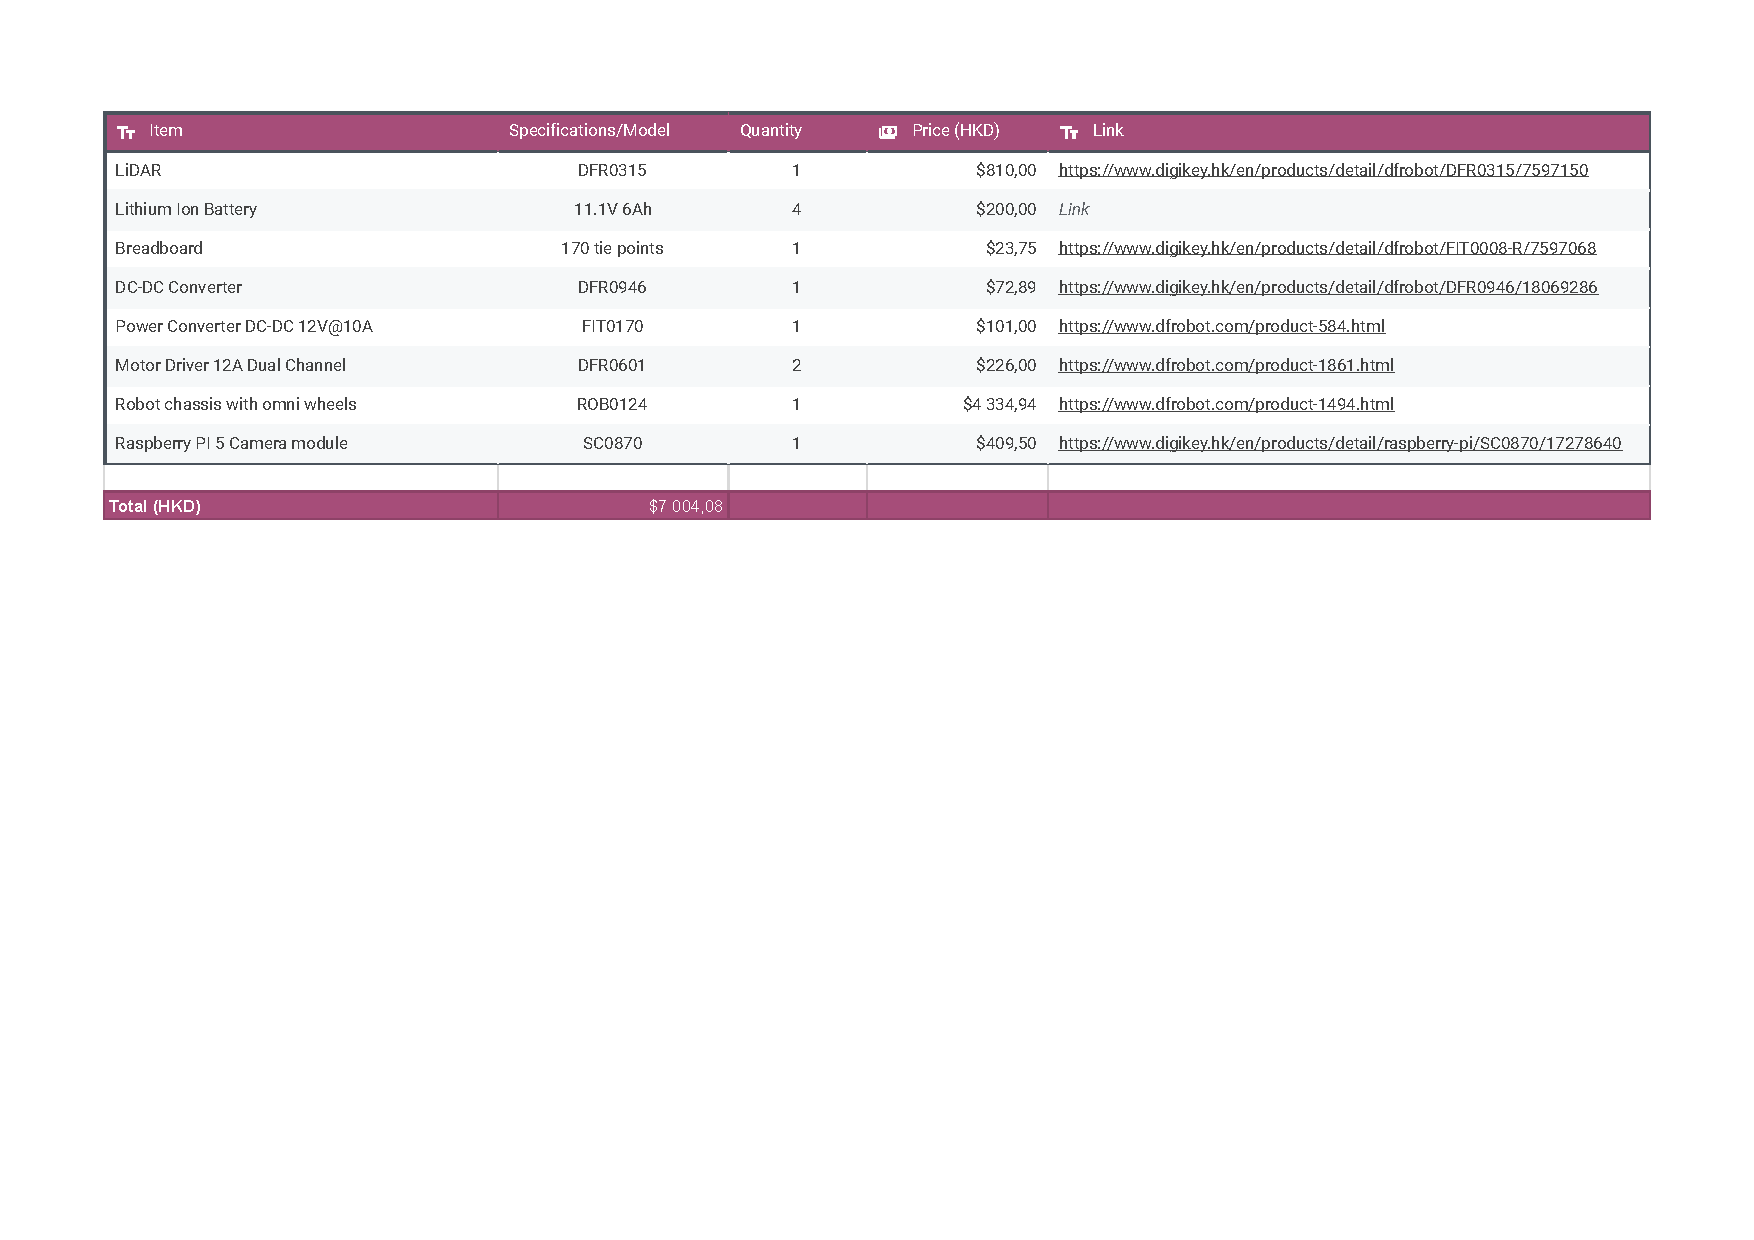
\includegraphics[width=\textwidth]{media/ProjectBudget - Arkusz2.pdf} % Placeholder for your block diagram image
    \vspace{-6cm}
    \caption{Component list with associated unit prices and quantities.}
    \label{table:budget}
\end{table}
\section{Conclusions}
In conclusion, the development of a nurse-following robot presents a promising solution to the critical nursing shortage in Hong Kong's healthcare system. Our project aims to enhance patient care efficiency by leveraging advanced technologies in robotics, navigation, tracking, and facial recognition. We successfully outlined a comprehensive plan that includes designing a self-mobile robot capable of omnidirectional movement, implementing an effective obstacle avoidance system, and integrating a robust person-tracking algorithm. The facial recognition system is designed to achieve high accuracy in identifying patients, which is crucial for ensuring safe and accurate medication administration.

The integration of these systems will not only streamline medication delivery processes but also alleviate the workload on nursing staff, allowing them to focus more on direct patient care. By addressing the engineering challenges identified in our literature review and utilizing modern computational tools like Raspberry Pi and ROS2, we are confident in our approach. As we move forward, continuous testing and refinement will be vital to ensure the robot's reliability and effectiveness in real hospital environments. This project has the potential to significantly improve healthcare delivery, and we look forward to its successful implementation and positive impact on patient care.
% References
\newpage
\phantomsection
\addcontentsline{toc}{section}{References}
\printbibliography


% Appendices
\newpage
\section*{Appendicies}
\phantomsection
\addcontentsline{toc}{section}{Appendix}

\subsection*{Appendix A—Meeting Minutes}

\textbf{Initial Meeting with Supervisor - 1 hour}

Date: 15/06/2024 \\
Time: 11:00 AM \\
Location: HKUST, ECE Commons \\
Attendees: Armaan, Wiktor, Ujaan, Professor Murch (Supervisor) \\
Minutes taken by: Armaan

\begin{itemize}
    \item The group introduced the idea of a robot capable of following a nurse in a hospital setting.
    \item Professor Murch provided feedback, suggesting starting with the tracking system and navigation before adding advanced features like facial recognition.
    \item Discussed potential tracking systems such as \textbf{UWB (Ultra-Wideband)} and \textbf{camera-based systems}.
    \item Armaan proposed using \textbf{omnidirectional wheels} for smooth movement, which was well received by the group.
    \item Professor Murch recommended using \textbf{ROS (Robot Operating System)} for software integration due to its modularity and community support.
    \item Basic ideas regarding motors and battery requirements were discussed, but no firm decisions were made.
\end{itemize}

\begin{table}[h]
    \centering
    \begin{tabular}{|c|c|c|}
        \hline
        \textbf{Action Item to be completed} & \textbf{By when} & \textbf{By whom} \\
        \hline
        Research tracking systems: UWB vs. Camera-based & 20/06/2024 & Ujaan \\
        \hline
        Draft initial robot design and chassis concept & 22/06/2024 & Armaan \\
        \hline
        Review ROS documentation for potential integration & 23/06/2024 & Wiktor \\
        \hline
        Set up project repository for code and documentation & 17/06/2024 & Ujaan \\
        \hline
        Follow up with Professor Murch on recommended motor specifications & 18/06/2024 & Armaan \\
        \hline
    \end{tabular}
    \caption{Action Items for Next Meeting}
    \label{tab:action_items_next_1}
\end{table}

\vspace{0.5cm}

\textbf{Follow-up Meeting and Presentation with Supervisor - 1 hour}

Date: 29/06/2024 \\
Time: 10:30 AM \\
Location: HKUST, ECE Commons \\
Attendees: Armaan, Wiktor, Ujaan, Professor Murch (Supervisor) \\
Minutes taken by: Ujaan

\begin{itemize}
    \item Followed up on previous meeting's actions. Ujaan completed research on tracking systems, Wiktor completed ROS review, Armaan still finalizing the chassis design.
    \item The team presented a basic overview of \textbf{ROS} and discussed tracking systems:
        \begin{itemize}
            \item \textbf{Camera-based object detection} vs. \textbf{tagging systems} (UWB or RFID). Pros and cons were discussed.
            \item Camera-based systems are flexible but could face occlusion challenges in crowded environments.
            \item Tag-based systems are reliable in crowded environments but less flexible for general-purpose tracking.
        \end{itemize}
    \item Armaan proposed using \textbf{Li-ion batteries} to balance size and capacity, aiming for a 1-hour battery life for initial testing.
    \item The team also discussed starting with a \textbf{basic object detection} test using a camera before finalizing the tracking system.
    \item Facial recognition and integration with a \textbf{mock patient database} were discussed but will be secondary focus.
    \item Division of labor was confirmed: 
        \begin{itemize}
            \item Armaan to focus on mechanical design (chassis and wheels).
            \item Wiktor to handle motor controllers and ROS integration.
            \item Ujaan to research tracking systems and power distribution.
        \end{itemize}
\end{itemize}

\begin{table}[h]
    \centering
    \begin{tabular}{|c|c|c|c|}
        \hline
        \textbf{Action Item to be completed} & \textbf{By when} & \textbf{By whom} & \textbf{Status} \\
        \hline
        Research tracking systems: UWB vs. Camera-based & 20/06/2024 & Ujaan & Completed \\
        \hline
        Draft initial robot design and chassis concept & 22/06/2024 & Armaan & In Progress \\
        \hline
        Review ROS documentation for potential integration & 23/06/2024 & Wiktor & Completed \\
        \hline
        Set up project repository for code and documentation & 17/06/2024 & Ujaan & Completed \\
        \hline
        Follow up with Professor Murch on recommended motor specifications & 18/06/2024 & Armaan & Completed \\
        \hline
    \end{tabular}
    \caption{Action Items from Previous Meeting}
    \label{tab:action_items_previous_2}
\end{table}

\begin{table}[h]
    \centering
    \begin{tabular}{|c|c|c|}
        \hline
        \textbf{Action Item to be completed} & \textbf{By when} & \textbf{By whom} \\
        \hline
        Begin basic object detection tests using a camera & 05/07/2024 & Ujaan \\
        \hline
        Finalize initial robot chassis design with selected wheels & 07/07/2024 & Armaan \\
        \hline
        Begin motor controller integration with ROS & 08/07/2024 & Wiktor \\
        \hline
        Investigate Kalman Filter or predictive algorithms for occlusion & 10/07/2024 & Ujaan \\
        \hline
        Research potential battery configurations and power requirements & 09/07/2024 & Armaan \\
        \hline
    \end{tabular}
    \caption{Action Items for Next Meeting}
    \label{tab:action_items_next_2}
\end{table}

\textbf{Proposal Planning - 4 hours}

Date: 04/09/2024 \\
Time: 12pm \\
Location: HKUST, ECE Commons \\
Attendees: Armaan, Wiktor, Ujaan \\
Minutes taken by: Ujaan Das

\begin{itemize}
    \item We met as a group on campus to discuss our objective statements and some specifics and will finalize most of them by the end of the week.
    \item Wiktor presented research on various hardware components such as Raspberry Pi and ROS. The group discussed the advantages of using ROS and minimal hardware, such as higher levels of abstraction and more modular components due to the aforementioned.
    \item Armaan discussed battery options and proposed using Li-ion batteries to balance size and capacity for longer operation. Anyhow, the group agreed on targeting a battery life of 1 hours for initial testing.
    \item Ujaan raised the need for a UWB-based tracking device for robust person-following in occluded environments. The group discussed potential integration challenges with the navigation system.
\end{itemize}

\begin{table}[h]
    \centering
    \begin{tabular}{|c|c|c|c|}
        \hline
        \textbf{Action Item} & \textbf{Due Date} & \textbf{Assigned To} & \textbf{Status} \\
        \hline
        Draft Introduction & 11/07/2024 & Armaan & In Progress \\
        \hline
        Complete Literature Review & 11/07/2024 & Wiktor, Ujaan & In Progress \\
        \hline
        Create Hardware Diagram & 11/07/2024 & Wiktor & In Progress \\
        \hline
        Create Software Diagram & 11/07/2024 & Armaan & In Progress \\
        \hline
        Create Gantt Chart & 11/07/2024 & Ujaan & In Progress \\
        \hline
    \end{tabular}
    \caption{Action Items for Proposal Development}
    \label{tab:proposal_action_items}
\end{table}

\begin{table}[h]
    \centering
    \begin{tabular}{|c|c|c|}
        \hline
        \textbf{Proposal Section} & \textbf{Assigned To} & \textbf{Due Date} \\
        \hline
        Introduction & Armaan & 11/07/2024 \\
        \hline
        Literature Review & Wiktor, Ujaan & 11/07/2024 \\
        \hline
        Hardware Diagram & Wiktor & 11/07/2024 \\
        \hline
        Software Diagram & Armaan & 11/07/2024 \\
        \hline
        Gantt Chart & Ujaan & 11/07/2024 \\
        \hline
    \end{tabular}
    \caption{Proposal Planning Timeline}
    \label{tab:proposal_planning_timeline}
\end{table}

\vspace{0.5cm}
% Meetings with Prof

\textbf{Pre-Proposal Submission Meeting with Supervisor - 30 minutes}

Date: 06/09/2024 \\
Time: 12pm \\
Location: ZOOM \\
Attendees: Prof. Ross Murch, Armaan, Wiktor, Ujaan \\
Minutes taken by: Wiktor Kowalczyk

\begin{itemize}
    \item We met with our project supervisor, Professor Murch, to discuss our progress in designing the system throughout the summer term.
    \item We discussed simplification of our initial design and setting realistic and achievable goals with metrics to quantify our solutions by.
    \item We discussed splitting the project into phases to take the advantage of the \textit{Divide-and-Conquer} approach for managing complexity.
\end{itemize}

\begin{table}[h]
    \centering
    \begin{tabular}{|c|c|c|c|}
        \hline
        \textbf{Action Item to be completed} & \textbf{By when} & \textbf{By whom} & \textbf{Status} \\
        \hline
        Introduction & 11/07/2024 & Armaan  & Completed\\
        \hline
        Literature Review  & 11/07/2024 & Wiktor, Ujaan & Completed\\
        \hline
        Hardware Diagram & 11/07/2024 & Wiktor  & Completed\\
        \hline
        Software Diagram  & 11/07/2024 & Armaan & Completed\\
        \hline
        Gantt Chart  & 11/07/2024 & Ujaan & Completed\\
        \hline
    \end{tabular}
    \caption{Action Items from Previous Meeting}
    \label{tab:action_items_previous}
\end{table}

\begin{table}[h]
    \centering
    \begin{tabular}{|c|c|c|}
        \hline
        \textbf{Action Item to be completed} & \textbf{By when} & \textbf{By whom} \\
        \hline
        Creation of precise budget and order list & 15/09/2024 & Wiktor, Armaan \\
        \hline
        Creation of high-level architecture for server-client in ROS2 & 15/09/2024 & Ujaan\\
        \hline
    \end{tabular}
    \caption{Action Items for Next Meeting}
    \label{tab:action_items_next}
\end{table}

%\subsection*{Appendix B (if necessary)}
%Further appendices may be included to present other relevant materials. DO NOT include any materials that should belong to the main body of the report.


\end{document}